%%%%%%%%%%%%%%%%%%%%%%%%%%%%%%%%%%%%%%%%%%%%%%%%%%%%%%%%%%%%%%%%%%%%%%%%%%%%%%%%
%% Plantilla de memoria en LaTeX para la ETSIT - Universidad Rey Juan Carlos
%%
%% Por Gregorio Robles <grex arroba gsyc.urjc.es>
%%     Grupo de Sistemas y Comunicaciones
%%     Escuela Técnica Superior de Ingenieros de Telecomunicación
%%     Universidad Rey Juan Carlos
%% (muchas ideas tomadas de Internet, colegas del GSyC, antiguos alumnos...
%%  etc. Muchas gracias a todos)
%%
%% La última versión de esta plantilla está siempre disponible en:
%%     https://github.com/gregoriorobles/plantilla-memoria
%%
%% Para obtener PDF, ejecuta en la shell:
%%   make
%% (las imágenes deben ir en PNG o JPG)

%%%%%%%%%%%%%%%%%%%%%%%%%%%%%%%%%%%%%%%%%%%%%%%%%%%%%%%%%%%%%%%%%%%%%%%%%%%%%%%%

\documentclass[a4paper, 12pt]{book}
%\usepackage[T1]{fontenc}

\usepackage[a4paper, left=2.5cm, right=2.5cm, top=3cm, bottom=3cm]{geometry}
\usepackage{times}
\usepackage[utf8]{inputenc}
%\usepackage[latin1]{inputenc}
%\usepackage[spanish]{babel} % Comenta esta l�nea si tu memoria es en ingl�s
\usepackage{url}
%\usepackage[dvipdfm]{graphicx}
\usepackage{graphicx}
\usepackage{float}  %% H para posicionar figuras
\usepackage[breaklinks=true]{hyperref} %% Para marcadores
\usepackage[nottoc, notlot, notlof, notindex]{tocbibind} %% Opciones de �ndice
\usepackage{latexsym}  %% Logo LaTeX
\usepackage{csquotes}  %% Paquete para citas (displayquote)
\usepackage{amsthm}  %% Paquete para Teoremas
\usepackage{color}  %% Paquete para texto en color
\usepackage[normalem]{ulem}  %% Para tablas
\useunder{\uline}{\ul}{}  %% Para tablas
\usepackage{listings}  %% para código y comandos
\definecolor{codegreen}{rgb}{0,0.6,0}
\definecolor{codegray}{rgb}{0.5,0.5,0.5}
\definecolor{codepurple}{rgb}{0.58,0,0.82}
\definecolor{backcolour}{rgb}{0.82,0.82,0.82}

\lstdefinestyle{mystyle}{
    backgroundcolor=\color{backcolour},
    commentstyle=\color{codegreen},
    keywordstyle=\color{magenta},
    numberstyle=\tiny\color{codegray},
    stringstyle=\color{codepurple},
    basicstyle=\ttfamily\footnotesize,
    breakatwhitespace=false,
    breaklines=true,
    captionpos=b,
    keepspaces=true,
    numbers=left,
    numbersep=5pt,
    showspaces=false,
    showstringspaces=false,
    showtabs=false,
    tabsize=2
}

\lstdefinestyle{mystylesmall}{
    backgroundcolor=\color{backcolour},
    commentstyle=\color{codegreen},
    keywordstyle=\color{magenta},
    numberstyle=\tiny\color{codegray},
    stringstyle=\color{codepurple},
    basicstyle=\ttfamily\scriptsize,
    breakatwhitespace=false,
    breaklines=true,
    captionpos=b,
    keepspaces=true,
    numbers=left,
    numbersep=5pt,
    showspaces=false,
    showstringspaces=false,
    showtabs=false,
    tabsize=2
}

\lstset{style=mystyle}

\title{Memoria del Proyecto}
\author{Miguel Ángel Fernández Sánchez}

\renewcommand{\baselinestretch}{1.5}  %% Interlineado

\begin{document}

%\renewcommand{\refname}{Bibliografía}  %% Renombrando
%\renewcommand{\appendixname}{Apéndice}

%%%%%%%%%%%%%%%%%%%%%%%%%%%%%%%%%%%%%%%%%%%%%%%%%%%%%%%%%%%%%%%%%%%%%%%%%%%%%%%%
% PORTADA

\begin{titlepage}
\begin{center}
\begin{tabular}[c]{c c}
%\includegraphics[bb=0 0 194 352, scale=0.25]{logo} &
\includegraphics[scale=0.25]{img/logo_vect.png} &
\begin{tabular}[b]{l}
\Huge
\textsf{UNIVERSIDAD} \\
\Huge
\textsf{REY JUAN CARLOS} \\
\end{tabular}
\\
\end{tabular}

\vspace{3cm}

\Large
GRADO INGENIERÍA SISTEMAS AUDIOVISUALES Y MULTIMEDIA

\vspace{0.4cm}

\large
Curso Académico 2017/2018

\vspace{0.8cm}

Trabajo Fin de Grado

\vspace{2.5cm}

\LARGE
HERRAMIENTA PARA ANALIZAR PROYECTOS FLOSS EN GITHUB (prov.)
% http://dl.acm.org/citation.cfm?id=2976778
\vspace{4cm}

\large
Autor : Miguel Ángel Fernández Sánchez \\
Tutor : Dr. Gregorio Robles
\end{center}
\end{titlepage}

\newpage
\mbox{}
\thispagestyle{empty} % para que no se numere esta pagina


%%%%%%%%%%%%%%%%%%%%%%%%%%%%%%%%%%%%%%%%%%%%%%%%%%%%%%%%%%%%%%%%%%%%%%%%%%%%%%%%
%%%% Para firmar
\clearpage
\pagenumbering{gobble}
\chapter*{Evaluation}

\vspace{-4cm}
\begin{center}
\LARGE
\textbf{Trabajo Fin de Grado}

\vspace{1cm}
\large
Herramienta para la extracción y el análisis de proyectos FLOSS en GitHub (provisional)

\vspace{1cm}
\large
\textbf{Autor :} Miguel Ángel Fernández Sánchez \\
\textbf{Tutor :} Dr. Gregorio Robles Martínez

\end{center}

\vspace{1cm}
La defensa del presente Trabajo Fin de Grado se realizó el día \qquad$\;\,$ de \qquad\qquad\qquad\qquad \newline de 20XX, siendo calificada por el siguiente tribunal:


\vspace{0.5cm}
\textbf{Presidente:}

\vspace{1.2cm}
\textbf{Secretario:}

\vspace{1.2cm}
\textbf{Vocal:}


\vspace{1.2cm}
y habiendo obtenido la siguiente calificación:

\vspace{1cm}
\textbf{Calificación:}


\vspace{1cm}
\begin{flushright}
Fuenlabrada, a \qquad$\;\,$ de \qquad\qquad\qquad\qquad de 20XX
\end{flushright}

%%%%%%%%%%%%%%%%%%%%%%%%%%%%%%%%%%%%%%%%%%%%%%%%%%%%%%%%%%%%%%%%%%%%%%%%%%%%%%%%
%%%% Dedicatoria

\chapter*{Dedications}
\pagenumbering{Roman} % para comenzar la numeracion de paginas en numeros romanos
\begin{flushright}
\textit{Dedicado a \\
mi familia / mi abuelo / mi abuela}
\end{flushright}

%%%%%%%%%%%%%%%%%%%%%%%%%%%%%%%%%%%%%%%%%%%%%%%%%%%%%%%%%%%%%%%%%%%%%%%%%%%%%%%%
%%%% Agradecimientos

\chapter*{Acknowledgements}
%\addcontentsline{toc}{chapter}{Agradecimientos} % si queremos que aparezca en el �ndice
\markboth{AGRADECIMIENTOS}{AGRADECIMIENTOS} % encabezado

Aquí vienen los agradecimientos\ldots Aunque esté bien acordarse de la pareja,
no hay que olvidarse de dar las gracias a tu madre, que aunque a veces no lo
parezca disfruta tanto de tus logros como tú\ldots Además, la pareja quizás
no sea para siempre, pero tu madre sí.


%%%%%%%%%%%%%%%%%%%%%%%%%%%%%%%%%%%%%%%%%%%%%%%%%%%%%%%%%%%%%%%%%%%%%%%%%%%%%%%%
%%%% Resumen en ingl�s

\chapter*{Summary}
%\addcontentsline{toc}{chapter}{Summary} % si queremos que aparezca en el �ndice
\markboth{SUMMARY}{SUMMARY} % encabezado

Here comes a translation of the ``Resumen'' into English. Please, double check
it for correct grammar and spelling. As it is the translation of the ``Resumen'',
which is supposed to be written at the end, this as well should be filled out
just before submitting.


%%%%%%%%%%%%%%%%%%%%%%%%%%%%%%%%%%%%%%%%%%%%%%%%%%%%%%%%%%%%%%%%%%%%%%%%%%%%%%%%
%%%% Resumen

\chapter*{Resumen}
%\addcontentsline{toc}{chapter}{Resumen} % si queremos que aparezca en el �ndice
\markboth{RESUMEN}{RESUMEN} % encabezado

Aquí viene un resumen del proyecto. Ha de constar de tres o cuatro párrafos,
donde se presente de manera clara y concisa de qué va el proyecto. Han
de quedar respondidas las siguientes preguntas:

\begin{itemize}
  \item ¿De qué va este proyecto? ¿Cuál es su objetivo principal?
  \item ¿Cómo se ha realizado? ¿Qué tecnologías están involucradas?
  \item ¿En qué contexto se ha realizado el proyecto? ¿Es un proyecto
dentro de un marco general?
\end{itemize}
Lo mejor es escribir el resumen al final.
%%%%%%%%%%%%%%%%%%%%%%%%%%%%%%%%%%%%%%%%%%%%%%%%%%%%%%%%%%%%%%%%%%%%%%%%%%%%%%%%
%%%%%%%%%%%%%%%%%%%%%%%%%%%%%%%%%%%%%%%%%%%%%%%%%%%%%%%%%%%%%%%%%%%%%%%%%%%%%%%%
% �NDICES %
%%%%%%%%%%%%%%%%%%%%%%%%%%%%%%%%%%%%%%%%%%%%%%%%%%%%%%%%%%%%%%%%%%%%%%%%%%%%%%%%

% Las buenas noticias es que los �ndices se generan autom�ticamente.
% Lo �nico que tienes que hacer es elegir cu�les quieren que se generen,
% y comentar/descomentar esa instrucci�n de LaTeX.

%%%% �ndice de contenidos
\tableofcontents
%%%% �ndice de figuras
\cleardoublepage
%\addcontentsline{toc}{chapter}{Lista de figuras} % para que aparezca en el indice de contenidos
\listoffigures % indice de figuras
%%%% �ndice de tablas
%\cleardoublepage
%\addcontentsline{toc}{chapter}{Lista de tablas} % para que aparezca en el indice de contenidos
%\listoftables % indice de tablas

%%%%%%%%%%%%%%%%%%%%%%%%%%%%%%%%%%%%%%%%%%%%%%%%%%%%%%%%%%%%%%%%%%%%%%%%%%%%%%%%
%%%%%%%%%%%%%%%%%%%%%%%%%%%%%%%%%%%%%%%%%%%%%%%%%%%%%%%%%%%%%%%%%%%%%%%%%%%%%%%%
% INTRODUCCI�N %
%%%%%%%%%%%%%%%%%%%%%%%%%%%%%%%%%%%%%%%%%%%%%%%%%%%%%%%%%%%%%%%%%%%%%%%%%%%%%%%%

\cleardoublepage
\chapter{Introduction}
\label{sec:intro} % etiqueta para poder referenciar luego en el texto con ~\ref{sec:intro}
\pagenumbering{arabic} % para empezar la numeraci�n de p�gina con n�meros
% En este cap�tulo se introduce el proyeto. Deber�a tener informaci�n general sobre
% el mismo, dando la informaci�n sobre el contexto en el �que se ha desarrollado.
% No te olvides de echarle un ojo a la p�gina con los cinco errores de escritura m�s frecuentes\footnote{\url{http://www.tallerdeescritores.com/errores-de-escritura-frecuentes}}.
% #TODO Ask for resources to back this data:
The way people develop software has evolved during these years: there is an extended social perception of developers to
being ingoing, solitary people, with very few social skills. But this sense is outdated: the paradigm has changed,
as coding has become almost a social activity. Developers who work collaborating with others produce better software [resource], as they
are continuously reading code from other developers, getting feedback about their contributions and consequently
widening their knowledge with new procedures and ideas. It turns out that this is how most of the software is produced nowadays,
so it is very difficult to become a successful developer without having good social skills.\\
If we think on social, virtual interactions among people, the first term that probably come to our minds will be
``\emph{Social networks}''. It is clear that those so-called social networks have produced a huge impact among a big part of the
population changing daily habits or affecting real-life relationships, just to name a few examples. As individuals, we share personal information every
day using interactive applications which allows us to participate somehow into a social network. Because of handling these
applications, we make specific interactions as users. \\
Let's see some examples. If we focus on Twitter, some of these interactions can be:
\begin{itemize}
    \item Following a Twitter user.
    \item \textit{Retweeting} a \textit{tweet} (propagate a message among all followers of the person who \textit{retweetted}).
    \item Using a \textit{hashtag} (a word preceded by a hash \# to label or classify a message into a topic).
\end{itemize}
\pagebreak Whereas on Facebook, we have other kinds of interactions:
\begin{itemize}
    \item Reacting to a post.
    \item Tagging a person in a picture.
    \item Writing a comment on someone's profile.
\end{itemize}
Talking about coding, in the last few years we have seen how this social trend came to software with the
emergence of social coding platforms, such as GitHub, BitBucket, GitLab, etc.\\
Social interactions in these platforms are about how software is developed and maintained but also how
contributions are managed (code review, continuous integration, etc.).\\
So, for example, on GitHub\footnote{\url{https://github.com}} we can find interactions like:
\begin{itemize}
    \item \textit{Forking} a repository (create an editable copy of a project).
    \item Seeing changes from last \textit{commit} (difference between most recent version and last version of the project).
    \item Checking the contributors of a repository.
    \item Submiting a \textit{Pull Request} (proposal to merge changes in a project).
\end{itemize}
These interactions that were mentioned, no matter their source, leave traces which remain stored in some computer on Earth.
This means we can obtain these data (though not all of it is publicly available) through the Internet using an \emph{API}
(\textit{Application programming interface}).\\
Once this information is retrieved, we can analyze it and extract conclusions about it.

\section{Free/Libre/Open-Source Software}
\label{sec:floss-definition}
In the following sections, we are going to talk about software and its development process, focusing on \emph{FLOSS} (Free/Libre, Open-source
software) projects, so it is inevitable to describe briefly what is this about.
During my degree, I was fortunate to be taught within \emph{FLOSS} values, as most of my professors plead
for Free/Libre software as their teaching model, by which I have obtained a distinctive knowledge and perspective as a professional but also as an individual.\\
\newpage
According to the \textbf{Free Software Foundation}\footnote{\url{https://www.gnu.org/philosophy/free-sw.html}}:
\begin{displayquote}
    \emph{Free software} means software that respects users' freedom and community. Roughly, it means that the users have the freedom
    to run, copy, distribute, study, change and improve the software. Thus, free software is a matter of liberty, not price. (\ldots)\\
    A program is free software if the program's users have the four essential freedoms:
       \begin{itemize}
           \item The freedom to run the program as you wish, for any purpose (freedom 0).
           \item The freedom to study how the program works, and change it so it does your computing as you wish (freedom 1).
           \item The freedom to redistribute copies (freedom 2).
           \item The freedom to distribute copies of your modified versions to others (freedom 3).
       \end{itemize}
    A program is free software if it gives users adequately all of these freedoms. Otherwise, it is \textit{nonfree}.
\end{displayquote}
% #TODO:
Due to the connotations which the word \emph{Free} has in English language (mentioned before), there is a definition
for \emph{Open source} software by the \textbf{Open Source Initiative}\footnote{\url{https://opensource.org/osd}} which
slighly varies from the \emph{FSF} definition. About this difference, Richard Stallman (founder of the \emph{FSF}) comments:
\begin{displayquote}
The term \emph{open source} software is used by some people to mean more or less the same category as free software.
It is not exactly the same class of software: they accept some licenses that we consider too restrictive,
and there are free software licenses they have not accepted. However, the differences in extension of the
category are small: nearly all free software is open source, and nearly all open source software is free.
\end{displayquote}
%Example code: \begin{verbatim}
\section{Motivation}
\label{sec:motivation}
I was working as a Researcher Assistant in \emph{GSyC/LibreSoft}\footnote{\url{http://www.libresoft.es}} department at Rey Juan Carlos University when I started to
deepen into Free/Libre software and the world of metrics. Then I had the great luck of start participating in a study that
Dr. Gregorio Robles was doing with researchers from Chalmers University in Gothenburg, Sweden. The main aim of their research was to
learn how \emph{UML} models\footnote{\url{http://uml.org/what-is-uml.htm}} are used in public \emph{FLOSS} projects (particularly, projects hosted on GitHub),
as most of the previous studies focused only on its industrial use.\\
Given the large size of GitHub as a platform and its access limitations, this research motivated to build a tool which extracts
data from all the existing repositories on GitHub, then filter those repositories which may include at least one
\emph{UML} model and finally analyze more in-depth the set of projects that meet this condition.\\\\
Since early stages of this research, this tool was designed and built using a modular structure, thought to be reusable
and adaptable to any kind of files that have to be found but also the way GitHub provides data; hoping to be useful
for other researches or any other person who might be interested on extract this information. Besides, the scale of this project
presented a personal challenge which provided me the opportunity to extend my knowledge and obtain a valuable point of
view about research and large-scope projects.
\section{Structure of the dissertation}
\label{sec:structure}
\textcolor{red}{(Work in progress)}\newline
During this dissertation, I am going to explain the different objectives that were stated for this project, the technology
which have been used to make it happen.\\
After that, I will detail the designing process and the tool architecture, itemizing on each one of its sections. Then,
we will explore the performance of the tool within a use case, taking into account the limitations and issues which arose
during it and how they were solved.\\Then, discuss about results from the use case and general conclusions
and to finish, consider future work and further steps for this project.
%%%%%%%%%%%%%%%%%%%%%%%%%%%%%%%%%%%%%%%%%%%%%%%%%%%%%%%%%%%%%%%%%%%%%%%%%%%%%%%%
%%%%%%%%%%%%%%%%%%%%%%%%%%%%%%%%%%%%%%%%%%%%%%%%%%%%%%%%%%%%%%%%%%%%%%%%%%%%%%%%
% OBJETIVOS %
%%%%%%%%%%%%%%%%%%%%%%%%%%%%%%%%%%%%%%%%%%%%%%%%%%%%%%%%%%%%%%%%%%%%%%%%%%%%%%%%
\cleardoublepage
\chapter{Objectives}
\label{sec:objectives}
It is widely known that GitHub allows to filter projects by a certain programming language (e.g.
\emph{Python}, \emph{C++}, etc.), but GitHub does not offer a mechanism through which you can identify projects
containing files with a certain extension or how many files match with some word or pattern in their
file-name in a repository. The fundamental research questions that motivated the creation of this tool were:
\begin{itemize}
  \item RQ1: How many GitHub repositories contain at least one file with a certain extension or a certain
        pattern in its file-name?
  \item RQ2: What is the history of those files in the life-span of the project?
\end{itemize}
Therefore, the main goal of this tool is to extract and analyze data from a set of GitHub projects in a scalable,
automated way in order to obtain quantitative information about the usage of a certain file type, programming language
or/and any search that can be expressed into patterns and heuristics.\\\\
Thus far, many studies focused in one single project or in a limited data-set when software development is analyzed, so
the next goal to define is to obtain the whole data-set of repositories hosted on all GitHub at a certain date.\\
For analyze the data from all GitHub in a proper way, we needed an static, reliable and updated source of this platform.\
This source is produced by the \emph{GHTorrent} project by a queriable, offline database with most of the information which the
GitHub \textit{API} can provide.\\
To finish answering \emph{RQ1}, we need to extract the list of files from the main branch [definition] of each repository so
it can be applied the different filters.\\\\
To answer to \emph{RQ2}, we need to analyze more in-depth marking those repositories with at least one positive result
after applying the filter, and then build a database with this extended data to extract useful information from it in a
systematic way.
%%%%%%%%%%%%%%%%%%%%%%%%%%%%%%%%%%%%%%%%%%%%%%%%%%%%%%%%%%%%%%%%%%%%%%%%%%%%%%%%
%%%%%%%%%%%%%%%%%%%%%%%%%%%%%%%%%%%%%%%%%%%%%%%%%%%%%%%%%%%%%%%%%%%%%%%%%%%%%%%%
% ESTADO DEL ARTE %
%%%%%%%%%%%%%%%%%%%%%%%%%%%%%%%%%%%%%%%%%%%%%%%%%%%%%%%%%%%%%%%%%%%%%%%%%%%%%%%%
\cleardoublepage
\chapter{State of the art}
\label{sec:state-art}
%Puedes citar libros, como el de Bonabeau et al. sobre procesos estigm�rgicos~\cite{bonabeau:_swarm}.
 % Nota que el ~ a�ade un espacio en blanco, pero no deja que exista un salto de l�nea. Imprescindible ponerlo para las citas.
\section{Python}
\label{sec:python}
\textbf{Python}\footnote{\url{https://www.python.org/}} is an interpreted, object-oriented, high-level, open source
programming language for general-purpose programming created by Guido van Rossum in 1991 (Nowadays, the most
recent version is 3.6.4, from December, 2017).\ Its design is focused on code readability and clear syntax, making
possible to program using fewer lines of code comparing to other programming languages as \emph{C++} or \emph{Ada}.\\
%Python is widely used over the world, for example: Numeric and Scientific Programming, ... \\
\emph{Python} features a large standard library, which includes many different tasks from text pattern matching to network
scripting, in addition to a vast collection of third-party application libraries.
Other remarkable features are portability, as \emph{Python} interpreters are available for many operating systems;
and the component integration, as \emph{Python} scripts can easily communicate with other parts of an application or code,
like \emph{C++} libraries, \emph{MySQL} databases, etc.\\
%As a downside to Python is that its execution speed may not always be as fast as a compiled, lower-level
%slanguages such as C and C++.\\
\section{Git}
\label{sec:git}
%source: https://git-scm.com/book/en/v2/Getting-Started-Git-Basics
\textbf{Git} is an open-source Version Control System (\emph{VCS}), originally developed in 2005 by Linus Torvalds.\
As any \emph{VCS}, \emph{git} is a system that records changes to a file or set of files over time
so that you can recall specific versions later.
It is by far, the most used \emph{VCS} in the world\footnote{\url{http://stackoverflow.com/research/developer-survey-2015}}.\\\\
The major difference between \emph{git} and any other VCS is the way \emph{git} thinks about its data.
Conceptually, most other systems store information as a list of file-based changes. Other systems like \textit{Subversion},
\textit{Perforce}, \textit{Bazaar}, etc. think of the information they store as a set of files and the changes made to each
file over time (See figure~\ref{fig:info-not-git}).\\
Instead, \emph{git} thinks of its data more like a series of snapshots of a miniature file-system (See figure~\ref{fig:info-not-git}).
With \emph{git}, every time you commit or save the state of your project, \emph{git} basically takes a picture of what all
your files look like at that moment and stores a reference to that snapshot. To be efficient, if files have not changed,
\emph{git} doesn't store the file again, just a link to the previous identical file it has already stored.
All this information is stored in a key-value system as \emph{git} objects, with a unique identity for each of them.
\subsection{Git objects definitions}
\label{ssec:git-definitions}
It is necessary to define some \emph{git} objects, as they are going to play a key role in this project.
\subsubsection{Commit}
A \textbf{commit} is a \emph{git} object which contains a record of the changes made to the repository since last modified
version of itself (last commit object). In the example in figure~\ref{fig:info-git}, each \textbf{commit} would be each different
\textit{Version} (1, 2, 3...), meaning that there is a new version of the repository with every \textbf{commit}.
\subsubsection{Tree}
A \emph{git} \textbf{tree} represents a directory and its structure (including file-names) in the repository, containing other possible
sub-directories as other child \textbf{tree} objects. However, these objects do not contain any information about the file contents:
that is stored in \textbf{blob} objects. In figure~\ref{fig:git-objs-example} there is an example of how \textbf{commits},
\textbf{trees} and \textbf{blobs} are connected with each other.
\subsubsection{Branch}
A \emph{git} \textbf{branch} is a pointer to a certain \emph{commit} object. All new commits
created from this pointer will diverge from the previous commit-history of the repository in two distinct, independent paths.
Branching is a very common and useful practice, as it allows to isolate different versions of the same files and directories
(but also different) in the same repository, and later, those branches can be merged into any other branch (See in
figure~\ref{fig:git-branches-example} a simplified example about the structure of a repository with several branches).
\begin{figure}
  \centering
  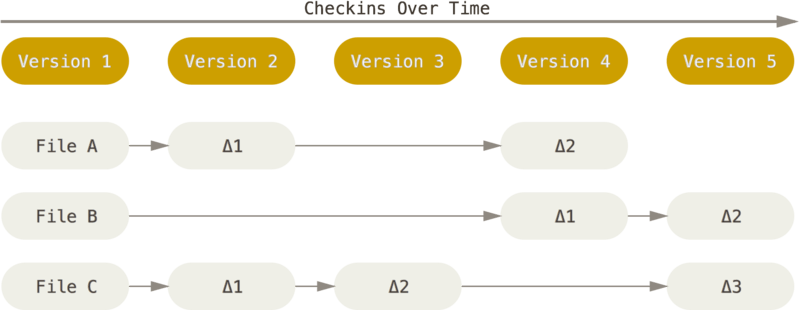
\includegraphics[width=12cm, keepaspectratio]{img/deltas-not-git}
  \caption{How other non-\emph{git} \emph{VCS} store information (Source: Git documentation).}
  \label{fig:info-not-git}
\end{figure}
\begin{figure}
  \centering
  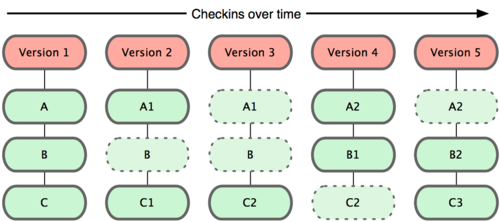
\includegraphics[width=12cm, keepaspectratio]{img/snapshots-git}
  \caption{How \emph{git} structures its information internally (Source: Git documentation).}
  \label{fig:info-git}
\end{figure}
\begin{figure}
  \centering
  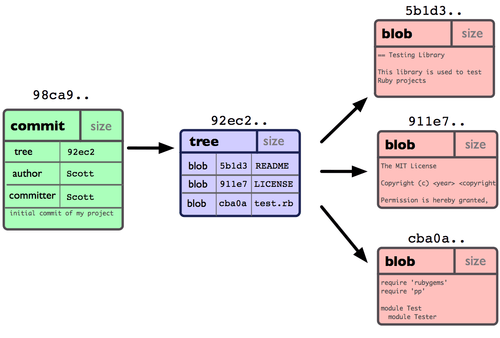
\includegraphics[width=12cm, keepaspectratio]{img/git-objs-example}
  \caption{Interaction among \textbf{commits}, \textbf{trees} and \textbf{blobs} (unique IDs above) (Source: Git documentation).}
  \label{fig:git-objs-example}
\end{figure}
\begin{figure}
  \centering
  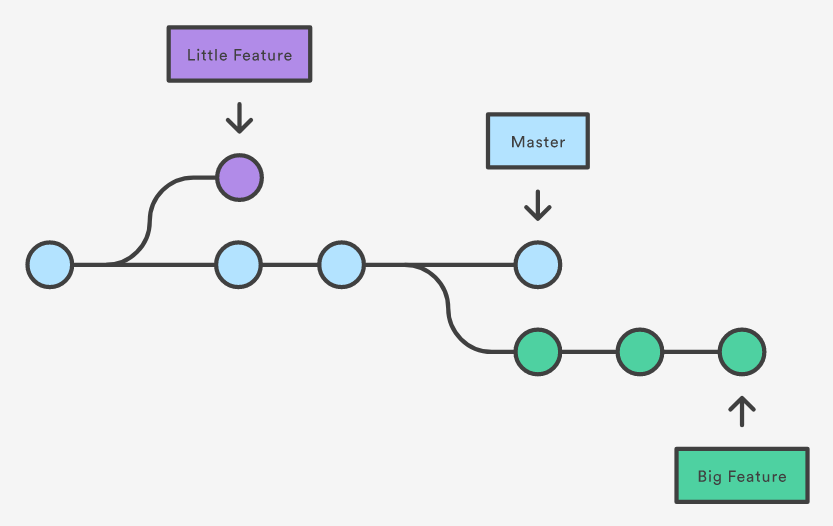
\includegraphics[width=12cm, keepaspectratio]{img/branches-example-atlassian}
  \caption{Abstraction of \emph{git} \textbf{branches} structure in a repository (Source: Atlassian).}
  \label{fig:git-branches-example}
\end{figure}
\section{GitHub}
\label{sec:github}
\textbf{GitHub} is a \emph{git}, web-based repository hosting service founded back in 2008. While \emph{git} is a command
line tool, GitHub provides a graphical interface, adding its own collaboration features such as a wikis and basic task
management tools for every project.\\
Each user on GitHub has their own profile, showing its past work and contributions to
other projects via \textit{pull requests}, \textit{forking} (create editable copies into someone's account) other repositories, etc.
Project revisions can be discussed publicly via \textit{issues} so many people can collaborate together to advance a project
forward. Currently, GitHub is the largest host of source code in the world,
with more than 124 million projects.
% TODO: https://www.quora.com/How-many-repositories-are-there-on-GitHub
%       https://www.howtogeek.com/180167/htg-explains-what-is-github-and-what-do-geeks-use-it-for/
%       https://techcrunch.com/2012/07/14/what-exactly-is-github-anyway/
\subsection{GitHub API}
\label{ssec:sec_gh-api}
%Should this definition be within a Glossary?
An \textbf{API} (\textit{Application Programming Interface}) is a set of subroutine definitions, protocols, and tools for building
application software. In general terms, it is a set of clearly defined methods of communication between various software components.\\\\
GitHub \textit{API} allows to access GitHub data, since own GitHub types like \textit{pull-requests}, \textit{issues} or \textit{forks}
to \emph{git}-related data, such as \textit{commits}, \textit{branches} or \textit{trees} using \textit{HTTP} requests and
returning information using \emph{JSON}(\textit{JavaScript Object Notation}) format.
\section{GHTorrent}
\label{sec:ghtorrent}
\begin{figure}
  \centering
  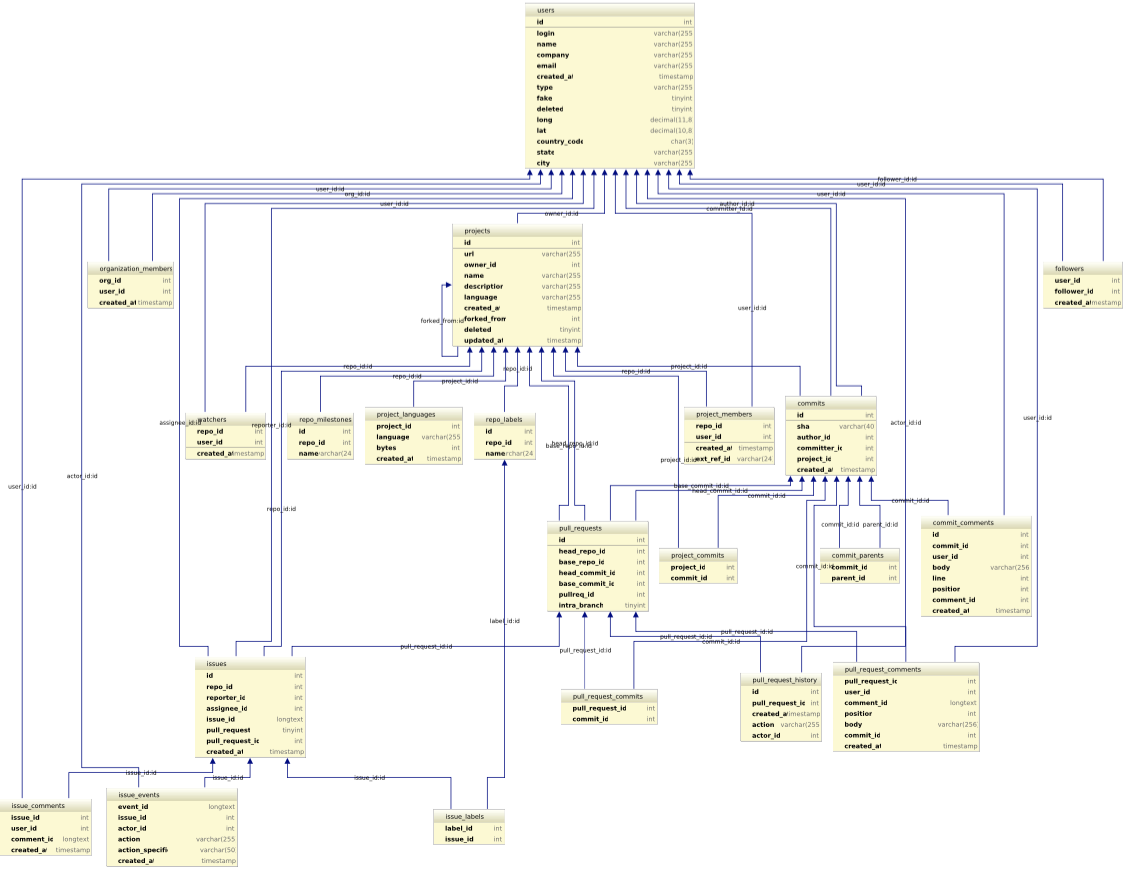
\includegraphics[width=16cm, keepaspectratio]{img/ghtorrent-schema}
  \caption{GHTorrent database relational schema}
  \label{fig:ghtorrent-schema}
\end{figure}
\textbf{GHTorrent} is a project based on create a scalable, queriable, offline mirror of data offered through the GitHub \textit{API}.\\
As they explain in their website\footnote{\url{http://ghtorrent.org/}}, \emph{GHTorrent} monitors the GitHub public event time line.
For each event, it retrieves its contents and their dependencies, exhaustively. Then, it stores the raw responses to a database whose
structure is represented in figure~\ref{ghtorrent-schema}.\
For each release, you can choose the \textit{dump} (a raw copy of a database) you want to download: either a \emph{MySQL} dump
(the full database, using one file per table) or a \emph{MongoDB} one (an incremental database).\\
\section{GrimoireLab and Perceval}
\label{sec:grimoire}
\textbf{GrimoireLab}\footnote{\url{http://grimoirelab.github.io/}} is a free, open source tool-set for software development analytics
mainly developed by the Spanish company \emph{Bitergia}\footnote{\url{https://bitergia.com/}}.
It allows you to retrieve data from many kinds of systems with information related to software development, and produce
analysis and visualizations with it.\\
We are focusing on a particular tool of \emph{GrimoireLab} called \textbf{Perceval}. This tool can retrieve data from more
than 20 different kinds of data sources, from \emph{git} repositories or GitHub projects, to issue trackers such as \emph{Jira}
or \emph{Bugzilla}, including messaging systems such as \emph{IRC}, \emph{Slack} or mailing lists, or other types of systems such as
\emph{StackOverflow} or \emph{Jenkins} in a regular and incremental way, allowing to produce uniform sets of information.
\newline \emph{GrimoireLab} is now part of \emph{CHAOSS}\footnote{\url{https://chaoss.community/}}, a project by \emph{The Linux Foundation}.
%%%%%%%%%%%%%%%%%%%%%%%%%%%%%%%%%%%%%%%%%%%%%%%%%%%%%%%%%%%%%%%%%%%%%%%%%%%%%%%%
%%%%%%%%%%%%%%%%%%%%%%%%%%%%%%%%%%%%%%%%%%%%%%%%%%%%%%%%%%%%%%%%%%%%%%%%%%%%%%%%
% DISEÑO E IMPLEMENTACIÓN %
%%%%%%%%%%%%%%%%%%%%%%%%%%%%%%%%%%%%%%%%%%%%%%%%%%%%%%%%%%%%%%%%%%%%%%%%%%%%%%%%
\cleardoublepage
\chapter{Design and implementation}
\label{sec:design-implementation}
This tool has a modular design, to ease its adaptability to future updates, changes on it dependencies or other needs which may appear.
The tool is divided into several linear sections with a set of \emph{Python} scripts, which can be grouped into three
main phases (See figure~\ref{fig:arquitectura}).
\begin{figure}
  \centering
  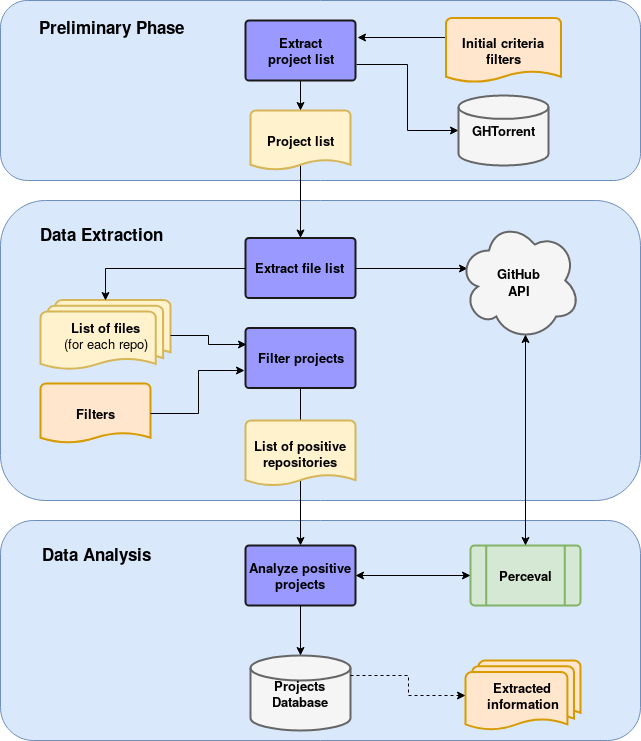
\includegraphics[width=12cm, keepaspectratio]{img/generic-tool-diagram-sections}
  \caption{General architecture of the tool}
  \label{fig:arquitectura}
\end{figure}
Before going into detail in each of these stages, let's introduce them briefly:
\begin{enumerate}
  \item \textbf{Preliminary phase}
    \begin{itemize}
      \item \textbf{Extract project list}:
            In this preliminary phase is where the list of GitHub repositories is retrieved. Using an offline dump of
            the \emph{GHTorrent} database, we get the \emph{project list} file containing all GitHub repositories from one of its tables
            and use a filter to choose among projects by their fields, like a major programming language, \textit{forked} or not, etc.
    \end{itemize}
  \item \textbf{Data extraction}
    \begin{itemize}
      \item \textbf{Extract file list}:
            This is the most critical section, because is where we obtain the main \textit{branch} and the file list
            (for each repository in the list from last section) querying the GitHub \textit{API}.
      \item \textbf{Filter projects}:
            It consists on iterating over the extracted file lists applying the corresponding patterns and heuristics.
            Then, it produces a \emph{list of positive results} file (repositories with at least one match).
    \end{itemize}
  \item \textbf{Data analysis}
    \begin{itemize}
      \item \textbf{Analyze positive projects}:
            Its function is to execute \emph{Perceval} with every project on the list of positive repositories
            building a \emph{projects database} which can be queried to extract information.
    \end{itemize}
\end{enumerate}
\section{Preliminary phase}
\label{sec:preliminary-phase}
% # TODO: https://growthhackers.com/growth-studies/github, https://blog.github.com/2013-12-23-10-million-repositories/
\begin{figure}
  \centering
  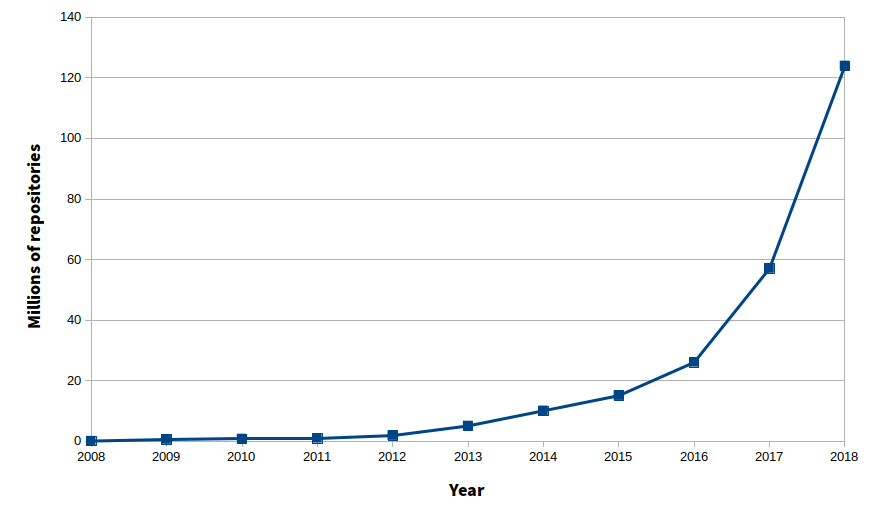
\includegraphics[width=14cm, keepaspectratio]{img/number-github-repos}
  \caption{Evolution of number of repositories on GitHub across time}
  \label{fig:total-repo-number}
\end{figure}
\begin{figure}
  \centering
  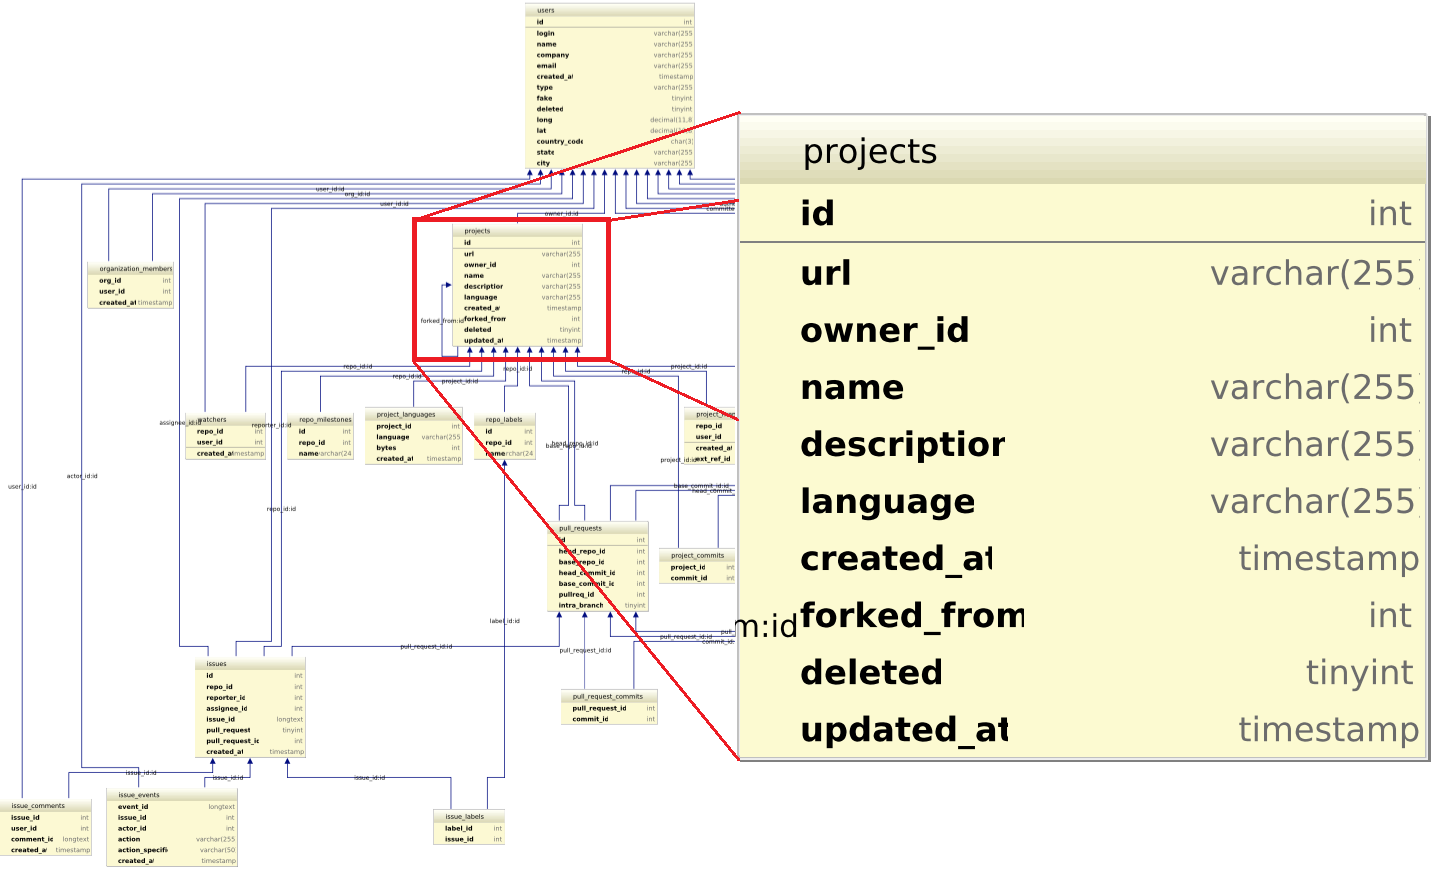
\includegraphics[width=16cm, keepaspectratio]{img/ghtorrent-schema-detail}
  \caption{\textit{Projects} table structure from GHTorrent database}
  \label{fig:ghtorrent-schema-detail}
\end{figure}
GitHub is the largest host of source code in the world (See figure~\ref{fig:total-repo-number} for a quantitative
estimation of GitHub scale evolution across time). Actually, the main problem we face is that there isn't a direct way
of obtaining the amount of GitHub repositories neither getting a list of them using its \textit{API}, so it is
very difficult to have quantitative and reliable data. For example, for building a graph like ~\ref{fig:total-repo-number},
its numbers had to be obtained directly from articles written by the GitHub team itself [\textcolor{red}{Source}]
and other people's estimations [\textcolor{red}{Source}].\\\\
At this point is where \emph{GHTorrent} project has its role in this story, as they provide an offline database dump with most
of the data which GitHub \textit{API} can provide at a certain date. This great collaborative effort is a huge advantage
for researchers, otherwise it would be practically non-viable retrieving full-scale GitHub data in a systematic way.
Nevertheless, it is important to mark that \emph{GHTorrent} database dump \underline{does not contain} \textit{Git trees}
(file-related) information: if this information was included, a major part of this tool (and by extension, this project) wouldn't
be necessary, as we could query and filter the data of our interest directly from the database which the \emph{GHTorrent} project provides.\\
If we have a look at how \emph{GHTorrent} database is structured (Figure~\ref{fig:ghtorrent-schema}), we can observe that
there is almost one table per GitHub object (\textit{users}, \textit{projects}, \textit{pull requests}, \textit{issues}, etc.).
Looking closer on these table's structure, we realize the table we need is the \emph{Projects} table
(see figure~\ref{fig:ghtorrent-schema-detail}), as it contains crucial repository-wise information including every project's name
and \textit{URL} but also other complementary information which could be used as a primary filter, like \texttt{language} (project's main language,
code-wise) or \texttt{forked\_from} (Empty if the repository isn't a \textit{fork} from another project), etc.\\\\
To obtain the actual data, the procedure to follow is:
\begin{enumerate}
  \item Download from \emph{GHTorrent} website a particular \emph{MySQL dump} which is provided as a compressed file in \texttt{tar.gz}
        format\footnote{To give an estimation of the current file sizes, the last dump available (2018, Mar 1st) sizes 71025 \texttt{MB}}.
  \item Uncompress the \texttt{tar.gz} file, which contains one \emph{CSV} file per table in the database.
  \item Get the file \texttt{projects.csv}, whose data corresponds to \emph{Projects} table (See an adapted\footnote{The field \emph{url} has been replaced by \emph{owner} to make the table more readable.}
  example of this file in table~\ref{table:projects-table-example}).
  \item Run the Python script \textcolor{red}{[reference to script]} with the corresponding filters to obtain the main
        \emph{project list} file, which will be the input for the next stage.
\end{enumerate}
Note that the filtering we establish in this phase is going to condition the results of our analysis. To make this task easier,
I decided to use a configuration file (See figure \textcolor{red}{[reference]}) to set basic filters and parameters. \textcolor{red}{(WIP)}\\
Finally, we obtain a filtered \emph{project list} file, which keeps the same format as \texttt{projects.csv} from the database dump.
\begin{table}[]
\centering
\caption{Adapted extract from \texttt{projects.csv} file, formatted as a table}
\label{table:projects-table-example}
\resizebox{\textwidth}{!}{%
\begin{tabular}{|c|c|c|c|c|c|c|c|c|c|}
\hline
\textbf{id} & \textbf{owner} & \textbf{owner\_id} & \textbf{name} & \textbf{descriptor} & \textbf{language} & \textbf{created\_at} & \textbf{forked\_from} & \textbf{deleted} & \textbf{updated\_at} \\ \hline
20 & chrisjaure & 80 & git-lava & Branching metaphor for git & Shell & 2012-02-27 02:45:44 &  -  & 0 & 2015-10-18 01:39:38 \\ \hline
21 & ES-DOC & 82 & django-cim-forms & - & Python & 2012-03-23 14:20:28 &  -  & 1 & 0000-00-00 00:00:00 \\ \hline
23 & adammark & 86 & Markup.js & Powerful JavaScript templates & JavaScript & 2011-08-23 00:30:04 &  -  & 0 & 2015-10-12 10:46:04 \\ \hline
24 & leoamigood & 88 & 1stdibs\_V2.1 & Initial setup with mule-pull project & Java & 2012-05-03 11:43:31 &  -  & 1 & 0000-00-00 00:00:00 \\ \hline
\end{tabular}%
}
\end{table}
\section{Data extraction}
\label{sec:data-extraction}
\begin{figure}
  \centering
  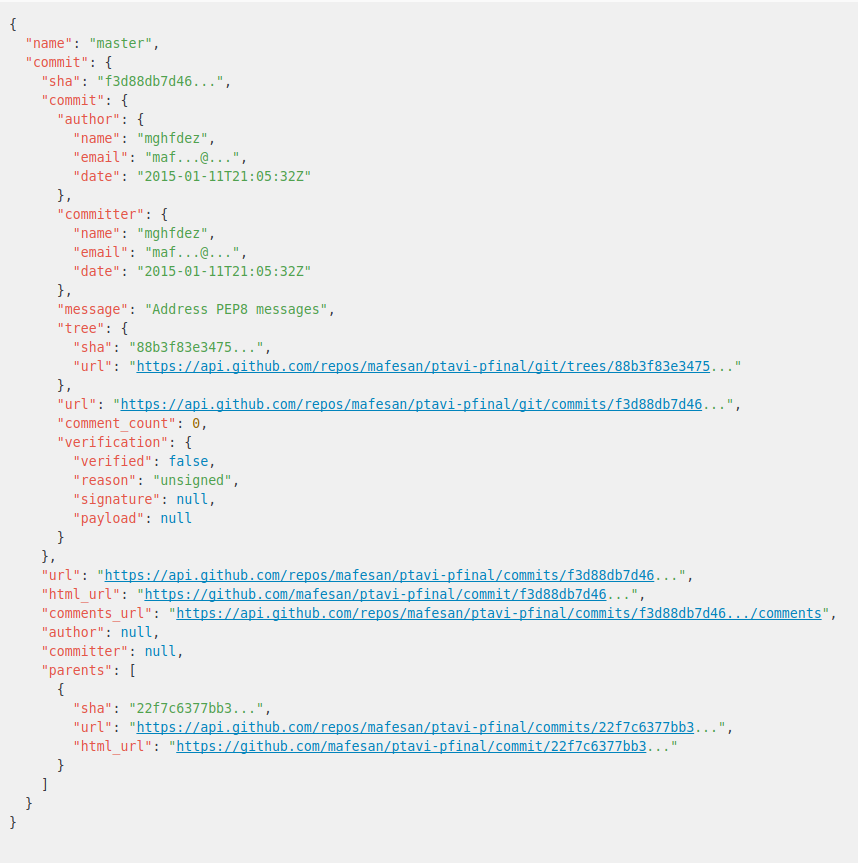
\includegraphics[width=13cm, keepaspectratio]{img/gh-api-master-json-example}
  \caption{Example: \texttt{JSON} response to the query asking for master branch data}
  \label{fig:gh-api-master-json}
\end{figure}
\begin{figure}
  \centering
  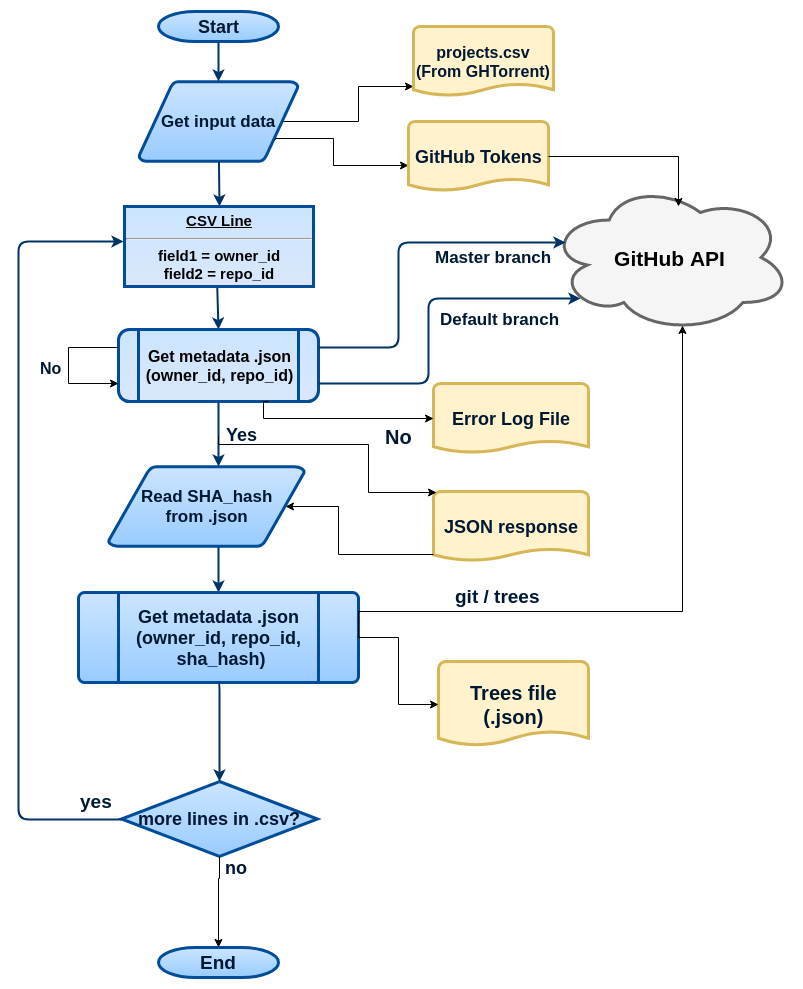
\includegraphics[width=14cm, keepaspectratio]{img/github-api}
  \caption{Flow-chart of \texttt{github-api.py} script}
  \label{fig:gh-api-diagram}
\end{figure}
Once the \emph{project list} file is ready, we can proceed to extract the file list of the main \textit{branch} of each
repository. To achieve this, we have to query the GitHub \textit{API} several times for each project.
It is important to mark this, as the GitHub \textit{API} has a limitation of 5.000 queries per hour for every authenticated
account, which caused a huge impact in the research and the data-retrieval process, as it is detailed in section (\textcolor{red}{Section}).\\\\
To make authenticated queries to the GitHub \textit{API} we need an \textbf{API token}. A \textbf{token} is a unique
identifier of an application requesting access to a service.
In the case of GitHub, they are long, alphanumeric strings of characters generated within a GitHub account,
so every executed action with that \textbf{token} is done on behalf of its owner's account.
For instance, if I want to \textit{fork} a repository into my GitHub account, I could do it either in two ways:
\begin{itemize}
  \item Log-in into my account, visit the repository \emph{URL} and press the \textbf{fork} button on GitHub's web interface.
  \item Send an authenticated \textit{query}\footnote{From now on, every time I refer to a GitHub \textit{API}
  request I will omit \texttt{https://api.github.com}.}
  to the GitHub \textit{API} like this one\footnote{On the requests, the parameters are marked with two dots (:).}:
  \begin{lstlisting}[language=bash]
  POST https://api.github.com/repos/:owner/:repo/forks?:token \end{lstlisting}
\end{itemize}
The script for this phase, \texttt{github-api.py} (See its diagram in figure~\ref{fig:gh-api-diagram}) has into account
this API limitation, ensuring that this limit is not exceeded. It employs three different directories in order to classify its outputs:
\textbf{master}, \textbf{default} and \textbf{trees}.
Then, it reads the \emph{project list} file and, per line, executes the following actions:
\begin{itemize}
  \item Check if the repository corresponding to that line has been downloaded before by looking at the existing files
  in the directories \textbf{master} or \textbf{default}.
  \item If not, try to obtain data from the \emph{master} \textit{branch}, whose output will be saved into the directory
  \textbf{master}.
  The \textit{query} sent to the GitHub \textit{API} to retrieve this data is:
  \begin{lstlisting}[language=bash]
  GET /repos/:owner/:repo/branches/master?:token \end{lstlisting}
  If we obtain a successful response, we will have a \texttt{JSON} file similar to the one in figure~\ref{fig:gh-api-master-json}.
  \item If the \emph{master} \textit{branch} is not found, we have to obtain the default \textit{branch} for that repository and
  perform another \textit{query} to retrieve the data from that \textit{branch}, which will be saved into the directory \textbf{default}.
  To retrieve this information, we need to obtain meta-data from the repository first and then, keep the content
  of the variable \texttt{default\_branch} to perform another \textit{query} to obtain data from that \textit{branch}:
  \begin{lstlisting}[language=bash]
  GET /repos/:owner/:repo?:token
  GET /repos/:owner/:repo/branches/:default_branch?:token \end{lstlisting}
  \item The last step is to read the obtained \texttt{JSON} data and get the tree objects recursively using the ID
  (\textit{SHA hash}) of the first one found in the response:
  \begin{lstlisting}[language=bash]
  GET /repos/:owner/:repo/git/trees/:sha?recursive=1&:token \end{lstlisting}
  This will be saved into the directory \textbf{trees}.
\end{itemize}
When this script finishes, we will have (assuming there were no errors) one \texttt{JSON} file per repository,
with the file-list information for the \textit{tree} objects in each repository.\\
However, the design of this script wouldn't be complete without considering all the possible errors and
particularities that may appear. Below, it is shown the most relevant setbacks and, if possible, an alternative
solution for every one of them:
\begin{itemize}
  \item \textbf{Private repository}. Some repositories in GitHub can be private if their owner hires a special
  plan on GitHub. The only solution is to perform the request with
  a token with granted access permissions to that repository, otherwise private repositories are ignored.
  \item \textbf{Truncated response}. Some repositories are too large so their tree and blob information is not completely
  sent within the response, but only a part of it and a Boolean field called \texttt{truncated} set to \texttt{True}.
  This was something that the GitHub \textit{API} implemented while we were performing the data retrieval of our
  use case, so we had to adapt the tool for it. The solution is to \textit{clone} (download) the repository,
  so later the next script can iterate locally over its files and folders.
  \item \textbf{Repository no longer exists}. There are repositories which existed at the time when that particular
  dump of the GHTorrent database was created, but they don't exist anymore.
  \item \textbf{\textit{Charset}-related errors}. Either the name of the repositories, owners, files, etc. can be written
  using different types of characters (Japanese, for instance) or other unknown characters (using another encoding)
  which sometimes caused encoding-decoding errors.
\end{itemize}
\section{Data filtering}
\label{sec:data-filtering}
\begin{figure}
  \centering
  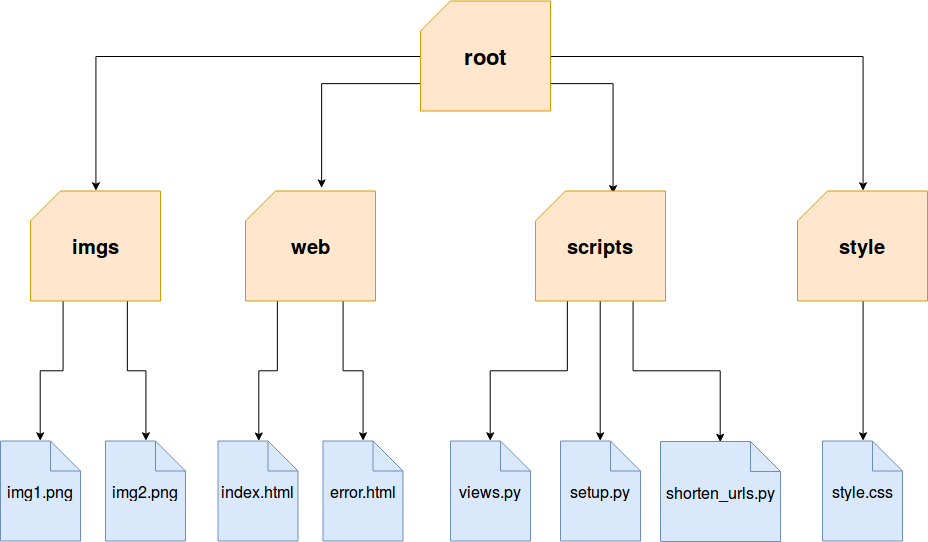
\includegraphics[width=13cm, keepaspectratio]{img/file-structure-example}
  \caption{Example: File-structure of a project to apply filters.}
  \label{fig:file-structure-example}
\end{figure}
\begin{figure}
  \centering
  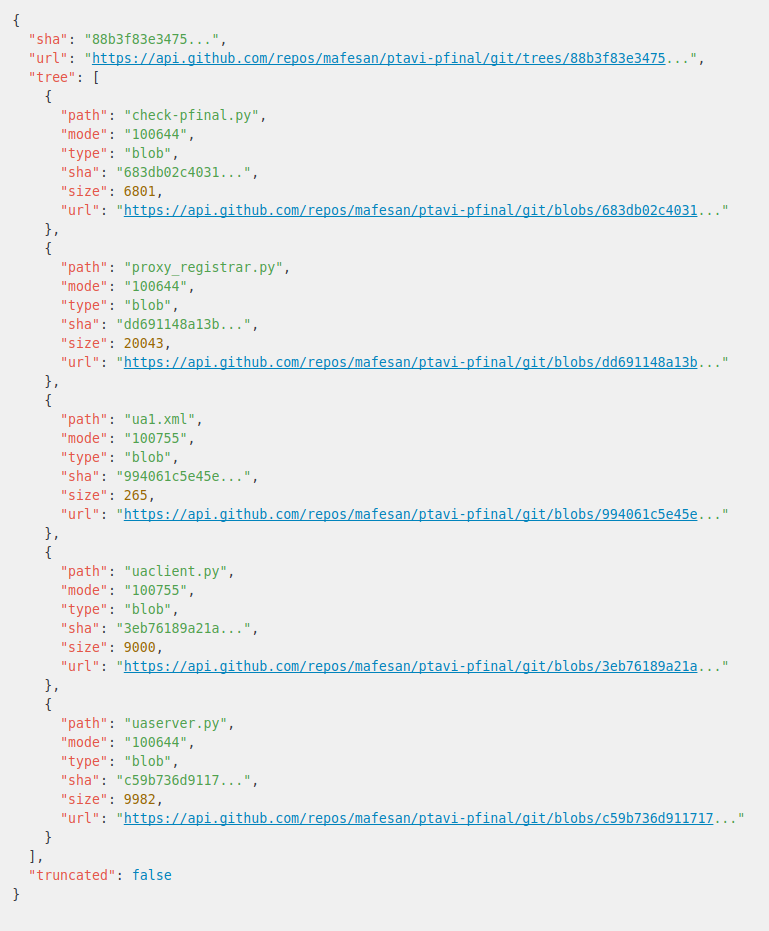
\includegraphics[width=13cm, keepaspectratio]{img/gh-api-trees-json-example}
  \caption{Example: \texttt{JSON} file containing information about \textit{tree} objects}
  \label{fig:gh-tree-json}
\end{figure}
\begin{figure}
  \centering
  \includegraphics[width=11cm, keepaspectratio]{img/github-tree}
  \caption{Flow-chart with the functioning of \texttt{github-tree.py} and \texttt{hits2urls.py} scripts.}
  \label{fig:gh-tree-diagram}
\end{figure}
\begin{table}[]
\centering
\caption{Example: definition of heuristics.}
\label{table:heuristics-table-example}
\begin{tabular}{|c|c|}
\hline
\textbf{Type of Heuristic} & \textbf{Pattern(s)}                                            \\ \hline
Level-1                    & \textit{.html}, \textit{.css}, \textit{.js}                    \\ \hline
Level-2                    & \textit{.py}                                                   \\ \hline
Key-words                  & \textit{urls}, \textit{views}, \textit{forms}, \textit{models} \\ \hline
\end{tabular}
\end{table}
\begin{table}[]
\centering
\caption{Positive results after applying heuristics filter.}
\label{table:heuristics-positive-example}
\begin{tabular}{|c|c|}
\hline
\textbf{Path}              & \textbf{Type of positive}   \\ \hline
scripts/shorten\_urls.py & Level-2 + contains key-word \\ \hline
scripts/views.py           & Level-2 + contains key-word \\ \hline
style/template.css         & Level-1                     \\ \hline
web/error.html             & Level-1                     \\ \hline
web/index.html             & Level-1                     \\ \hline
\end{tabular}
\end{table}
In this section is where the data we have obtained from the previous stage is filtered according to our search.
The approach that have been followed to apply filters is to define three types of heuristics, related to
file extensions and keywords:
\begin{itemize}
  \item \textbf{Level-1} file extensions, those which are a top priority in our search. They are immediately considered
   as positive results.
  \item \textbf{Level-2} file extensions, marked as relevant only if they meet one or more additional conditions.
  \item \textbf{Key-words}, specific words or groups of characters which a file-name with a \textit{Level-2} extension
  has to contain to be considered as a positive result.
\end{itemize}
Let's imagine a basic example where we are interested in projects related with web development. Defining the
necessary heuristics as in table~\ref{table:heuristics-table-example}, we will keep any file whose extension
is on Level-1 list, and those files whose extension is on Level-2 list \textbf{AND} whose file-name contains at least one
of the words (or group of characters) defined in the key-word list.\\
\begin{itemize}
  \item \texttt{.html} is on \textbf{Level-1} list, so any file with \texttt{html} extension will be a positive result directly.
  \item \texttt{.py} is on \textbf{Level-2} list, so only \texttt{.py} files containing at least one key-word in their file-name
  (i.e. \textit{urls}) will be considered as a positive result.
\end{itemize}
To complete this example, if we apply this filter to a repository whose file structure is like the one in figure~\ref{fig:file-structure-example},
we would obtain the set of positive results showed at table~\ref{table:heuristics-positive-example}.\\\\
Now, the next step is applying these filters to the \texttt{JSON} files which have been obtained before.
Specifically, we are interested only in those files included into the \textbf{trees} directory.
Each of those files contains the file structure of the last version of its repository,
where the \textit{tree} object contains under itself all the files (\textit{blob} objects) and sub-directories
(other \textit{tree} objects). Every object, no matter if it is a \textit{tree} or a \textit{blob}, contains the following parameters:
\begin{itemize}
  \item \textbf{path}: Absolute path of that file or folder inside the repository.
  \item \textbf{mode}: This number shows file mode information (file type, permissions, etc.) using UNIX notations.
  \item \textbf{type}: This value will be \texttt{blob} if it is a file, or \texttt{tree} if it is a folder.
  \item \textbf{sha}: Unique identifier for that \emph{git} object.
  \item \textbf{size}: File size in \textit{bytes}. Only \texttt{blob} objects contain this parameter.
  \item \textbf{url}: Link to this object in GitHub \textit{API}.
\end{itemize}
There is a simple example of the content of one of these files at figure~\ref{fig:gh-tree-json}.\\\\
The corresponding scripts for this phase are \texttt{github-tree.py} and \texttt{hits2urls.py}
(See a diagram for both of them in figure~\ref{fig:gh-tree-diagram}):\\
\texttt{github-tree.py} iterates over all the \texttt{JSON} files in the \textbf{trees} directory,
executing these simple instructions per file:
\begin{itemize}
  \item Load \texttt{JSON} data into a \emph{Python} \textit{dictionary} (a key-value data structure).
  \item Obtain the parent \texttt{tree} object (field \texttt{"tree"} in our \textit{dictionary}).
  \item Check the \texttt{"type"} field for every child object.
  \item If its type is \texttt{"blob"}, apply the pre-defined patterns and heuristics.
  \item Provide the positive results printing every matching object's \texttt{"path"} and \texttt{"URL"}.
\end{itemize}
\texttt{hits2urls.py} is a simple script which converts every \texttt{URL} from the last script (links to \texttt{blob} objects
in the GitHub \textit{API}), to the \texttt{URL} for the actual file which that object is representing to.
Here is an example of one \texttt{URL} which belongs to a \texttt{blob} object converted to the \texttt{URL}
pointing to the actual file (see below lines 1 and 2, respectively):
\begin{lstlisting}[language=bash]
https://api.github.com/repos/mafesan/ptavi-pfinal/git/blobs/3eb76189a21a...
https://raw.githubusercontent.com/mafesan/ptavi-pfinal/master/uaclient.py \end{lstlisting}
\section{Data analysis}
\label{sec:data-analysis}
In this section is where the positive results are analysed deeply to end up building a database to store
all the extracted information so it can be queried to perform our desired analysis.
\subsection{Extract extended repository information}
\label{ssec:extract-perceval}
To analyze the resulting repositories we take advantage of \textbf{Perceval}, a mature, powerful tool which
is capable of retrieving data from more than 25 different data sources producing a uniform set of data which can be
updated along time.\\
The data sources which Perceval supports are given by its \emph{backends}, and we are using the \emph{Git backend} to
obtain Git-related information from those GitHub repositories with at least one positive result.
Perceval clones repository by repository and parses every Git event log, producing a \emph{JSON} file
per repository containing data for every commit and its related Git objects.\\
\subsection{Building the database}
\label{ssec:build-database}
Next step is to build a database, which allows to store the extracted data in an optimized way to
obtain elaborated results by using queries according to our case of study.\\
As we had used the GHTorrent database, which is a MySQL database, we decided to use a MySQL database
for this purpose too, as it is easier to build and maintain.
We designed this database to contain five tables; four of them using data from the files which are obtained with
\textbf{Perceval} and one table from the GHTorrent database, \texttt{USERS} containing information about GitHub user accounts.
These tables and their full structure are in figure \textcolor{red}{(ref)}, and as a summary, these tables contain the following information:
\begin{itemize}
  \item \texttt{REPOS}: For a repository; its name, number of commits, URL, founder, etc.
  \item \texttt{PEOPLE}: Referring to the people who authored the commits, their name and email.
  \item \texttt{COMMITS}: For each commit object; its ID in Git, its ID on GitHub, which repository belongs to, ID of its author, etc.
  \item \texttt{INTERESTING\_FILES}: For each file (positive result); its name, URL, which repository belongs to and which commits this file is included into.
  \item \texttt{USERS}: From GHTorrent, GitHub user account information as login, name, location, company, creation date, etc.
\end{itemize}
\subsection{Querying the database}
\label{ssec:query-database}
Once the database has been build and filled with the data, to produce proper results for our analysis we have to ensure
that the perform the right queries.\\
Here are some standard queries we can execute to perform a basic analysis:
\begin{itemize}
  \item Query 1 (tentative)
  \begin{lstlisting}[language=SQL]
  SELECT (*) FROM users; \end{lstlisting}
\end{itemize}
%%%%%%%%%%%%%%%%%%%%%%%%%%%%%%%%%%%%%%%%%%%%%%%%%%%%%%%%%%%%%%%%%%%%%%%%%%%%%%%%
%%%%%%%%%%%%%%%%%%%%%%%%%%%%%%%%%%%%%%%%%%%%%%%%%%%%%%%%%%%%%%%%%%%%%%%%%%%%%%%%
% RESULTADOS %
%%%%%%%%%%%%%%%%%%%%%%%%%%%%%%%%%%%%%%%%%%%%%%%%%%%%%%%%%%%%%%%%%%%%%%%%%%%%%%%%
\cleardoublepage
\chapter{Results}
\section{Case of study: UML}
\label{sec:case-study-uml}
%%%%%%%%%%%%%%%%%%%%%%%%%%%%%%%%%%%%%%%%%%%%%%%%%%%%%%%%%%%%%%%%%%%%%%%%%%%%%%%%
%%%%%%%%%%%%%%%%%%%%%%%%%%%%%%%%%%%%%%%%%%%%%%%%%%%%%%%%%%%%%%%%%%%%%%%%%%%%%%%%
% CONCLUSIONES %
%%%%%%%%%%%%%%%%%%%%%%%%%%%%%%%%%%%%%%%%%%%%%%%%%%%%%%%%%%%%%%%%%%%%%%%%%%%%%%%%
\cleardoublepage
\chapter{Conclusions}
\label{chap:conclusions}
\section{Achieved objectives}
\label{sec:achieved-objectives}
Esta sección es la sección espejo de las dos primeras del capítulo de objetivos,
donde se planteaba el objetivo general y se elaboraban los específicos.
Es aquí donde hay que debatir qué se ha conseguido y qué no. Cuando algo no
se ha conseguido, se ha de justificar, en términos de qué problemas se han
encontrado y qué medidas se han tomado para mitigar esos problemas.
\section{Knowledge application}
\label{sec:knowledge-application}
Aquí viene lo que has aprendido durante el Grado/Máster y que has aplicado
en el TFG/TFM. Una buena idea es poner las asignaturas más relacionadas y
comentar en un párrafo los conocimientos y habilidades puestos en práctica.
\subsection{Related courses}
\begin{itemize}
  \item Informática 1
  \item Informática 2
  \item Arquitectura de Internet
  \item Sistemas Telemáticos para medios audiovisuales
  \item Protocolos de Transmisión de Audio y Video en Internet
  \item Laboratorio de Tecnologías Audiovisuales en la Web
\end{itemize}
\section{Learning outcomes}
\label{sec:learning-outcomes}
Aquí viene lo que has aprendido en el Trabajo Fin de Grado/Máster.
\begin{enumerate}
  \item a
  \item b
\end{enumerate}
\section{Future work}
\label{sec:future-work}
Ningún software se termina, así que aquí vienen ideas y funcionalidades
que estaría bien tener implementadas en el futuro.
Es un apartado que sirve para dar ideas de cara a futuros TFGs/TFMs.
\section{Personal assessment}
\label{sec:assessment}
Finalmente (y de manera opcional), hay gente que se anima a dar su punto de
vista sobre el proyecto, lo que ha aprendido, lo que le gustaría haber aprendido,
las tecnologías utilizadas y demás.
%%%%%%%%%%%%%%%%%%%%%%%%%%%%%%%%%%%%%%%%%%%%%%%%%%%%%%%%%%%%%%%%%%%%%%%%%%%%%%%%
%%%%%%%%%%%%%%%%%%%%%%%%%%%%%%%%%%%%%%%%%%%%%%%%%%%%%%%%%%%%%%%%%%%%%%%%%%%%%%%%
% AP�NDICE(S) %
%%%%%%%%%%%%%%%%%%%%%%%%%%%%%%%%%%%%%%%%%%%%%%%%%%%%%%%%%%%%%%%%%%%%%%%%%%%%%%%%
\cleardoublepage
\appendix
\chapter{User manual}
\label{app:manual}
\chapter{Published papers}
\label{app:papers}
%%%%%%%%%%%%%%%%%%%%%%%%%%%%%%%%%%%%%%%%%%%%%%%%%%%%%%%%%%%%%%%%%%%%%%%%%%%%%%%%
%%%%%%%%%%%%%%%%%%%%%%%%%%%%%%%%%%%%%%%%%%%%%%%%%%%%%%%%%%%%%%%%%%%%%%%%%%%%%%%%
% BIBLIOGRAFIA %
%%%%%%%%%%%%%%%%%%%%%%%%%%%%%%%%%%%%%%%%%%%%%%%%%%%%%%%%%%%%%%%%%%%%%%%%%%%%%%%%
\cleardoublepage
% Las siguientes dos instrucciones es todo lo que necesitas
% para incluir las citas en la memoria
\bibliographystyle{abbrv}
\bibliography{memoria}  % memoria.bib es el nombre del fichero que contiene
% las referencias bibliogr�ficas. Abre ese fichero y mira el formato que tiene,
% que se conoce como BibTeX. Hay muchos sitios que exportan referencias en
% formato BibTeX. Prueba a buscar en http://scholar.google.com por referencias
% y ver�s que lo puedes hacer de manera sencilla.
% M�s informaci�n:
% http://texblog.org/2014/04/22/using-google-scholar-to-download-bibtex-citations/
\end{document}
